\documentclass{article}
\usepackage[utf8]{inputenc}
\usepackage{graphicx}
\graphicspath{ {./images/} }
\usepackage{amsmath}
\usepackage{graphicx} % for figures
\usepackage{float} % figure placement
\usepackage{fancyhdr}
\usepackage{hyperref}

\hypersetup{
    colorlinks=true,
    linkcolor=blue,
    filecolor=magenta,      
    urlcolor=cyan,
    pdftitle={Overleaf Example},
    pdfpagemode=FullScreen,
}

\title{The Inter-connectivity of the TCAT System; Networks with Eigenvalues and Eigenvectors}

\author{Ming DeMers}
\date{March 2022}

\begin{document}
\def\ind{\hspace*{0.3in}}
	\def\gap{0.2in}
%add a header and footer
\pagestyle{fancy}
\lhead{Ming DeMers}
\rhead{March 23, 2022}
\chead{Inter-connectivity of the TCAT System}
\cfoot{\thepage}
\renewcommand{\headrulewidth}{0.4pt}
\renewcommand{\footrulewidth}{0.4pt}

\section{Introduction}
Originating from three separate transit systems, the Tompkins Consolidated Area Transit (TCAT) System connects many popular locations in Ithaca and Tompkins County by a number of bus routes. This project examines the inter-connectivity of the TCAT system by visualizing and analyzing the routes and the amount of connections by which certain popular locations can be reached. 

\section{Network Description and Sources}
The network studied here is the TCAT system as of Spring 2022. The network was sourced by the TCAT website and its section on "popular destinations."[1] Each node represents the location of a bus stop and each edge indicates how many routes serve that route. Fifteen locations, representing nodes, were chosen based on factors of frequent use, necessity, and personal judgement. Locations served by identical routes and were close to each other were omitted to discourage duplicate data. Residential areas were omitted for simplicity. 
\\
\\
1. \emph{Popular Destinations}, Tompkins Consolidated Area Transit Inc., 2022. tcatbus.com /ride/popular-destinations/

\section{Laplacian Matrix and Network Representation}
There are a total of 15 nodes within this network. Each node is labeled with its name and each edge shows the route number. Each edge connects two locations, representing that these two stops are within the same route, and can be reached thereof. The result is the 15-node, 62-edge network shown below. Moreover, a resulting subset of the Laplacian matrix L is shown next to it, showing the first 10 rows and columns for simplicity.


\begin{figure}[t]
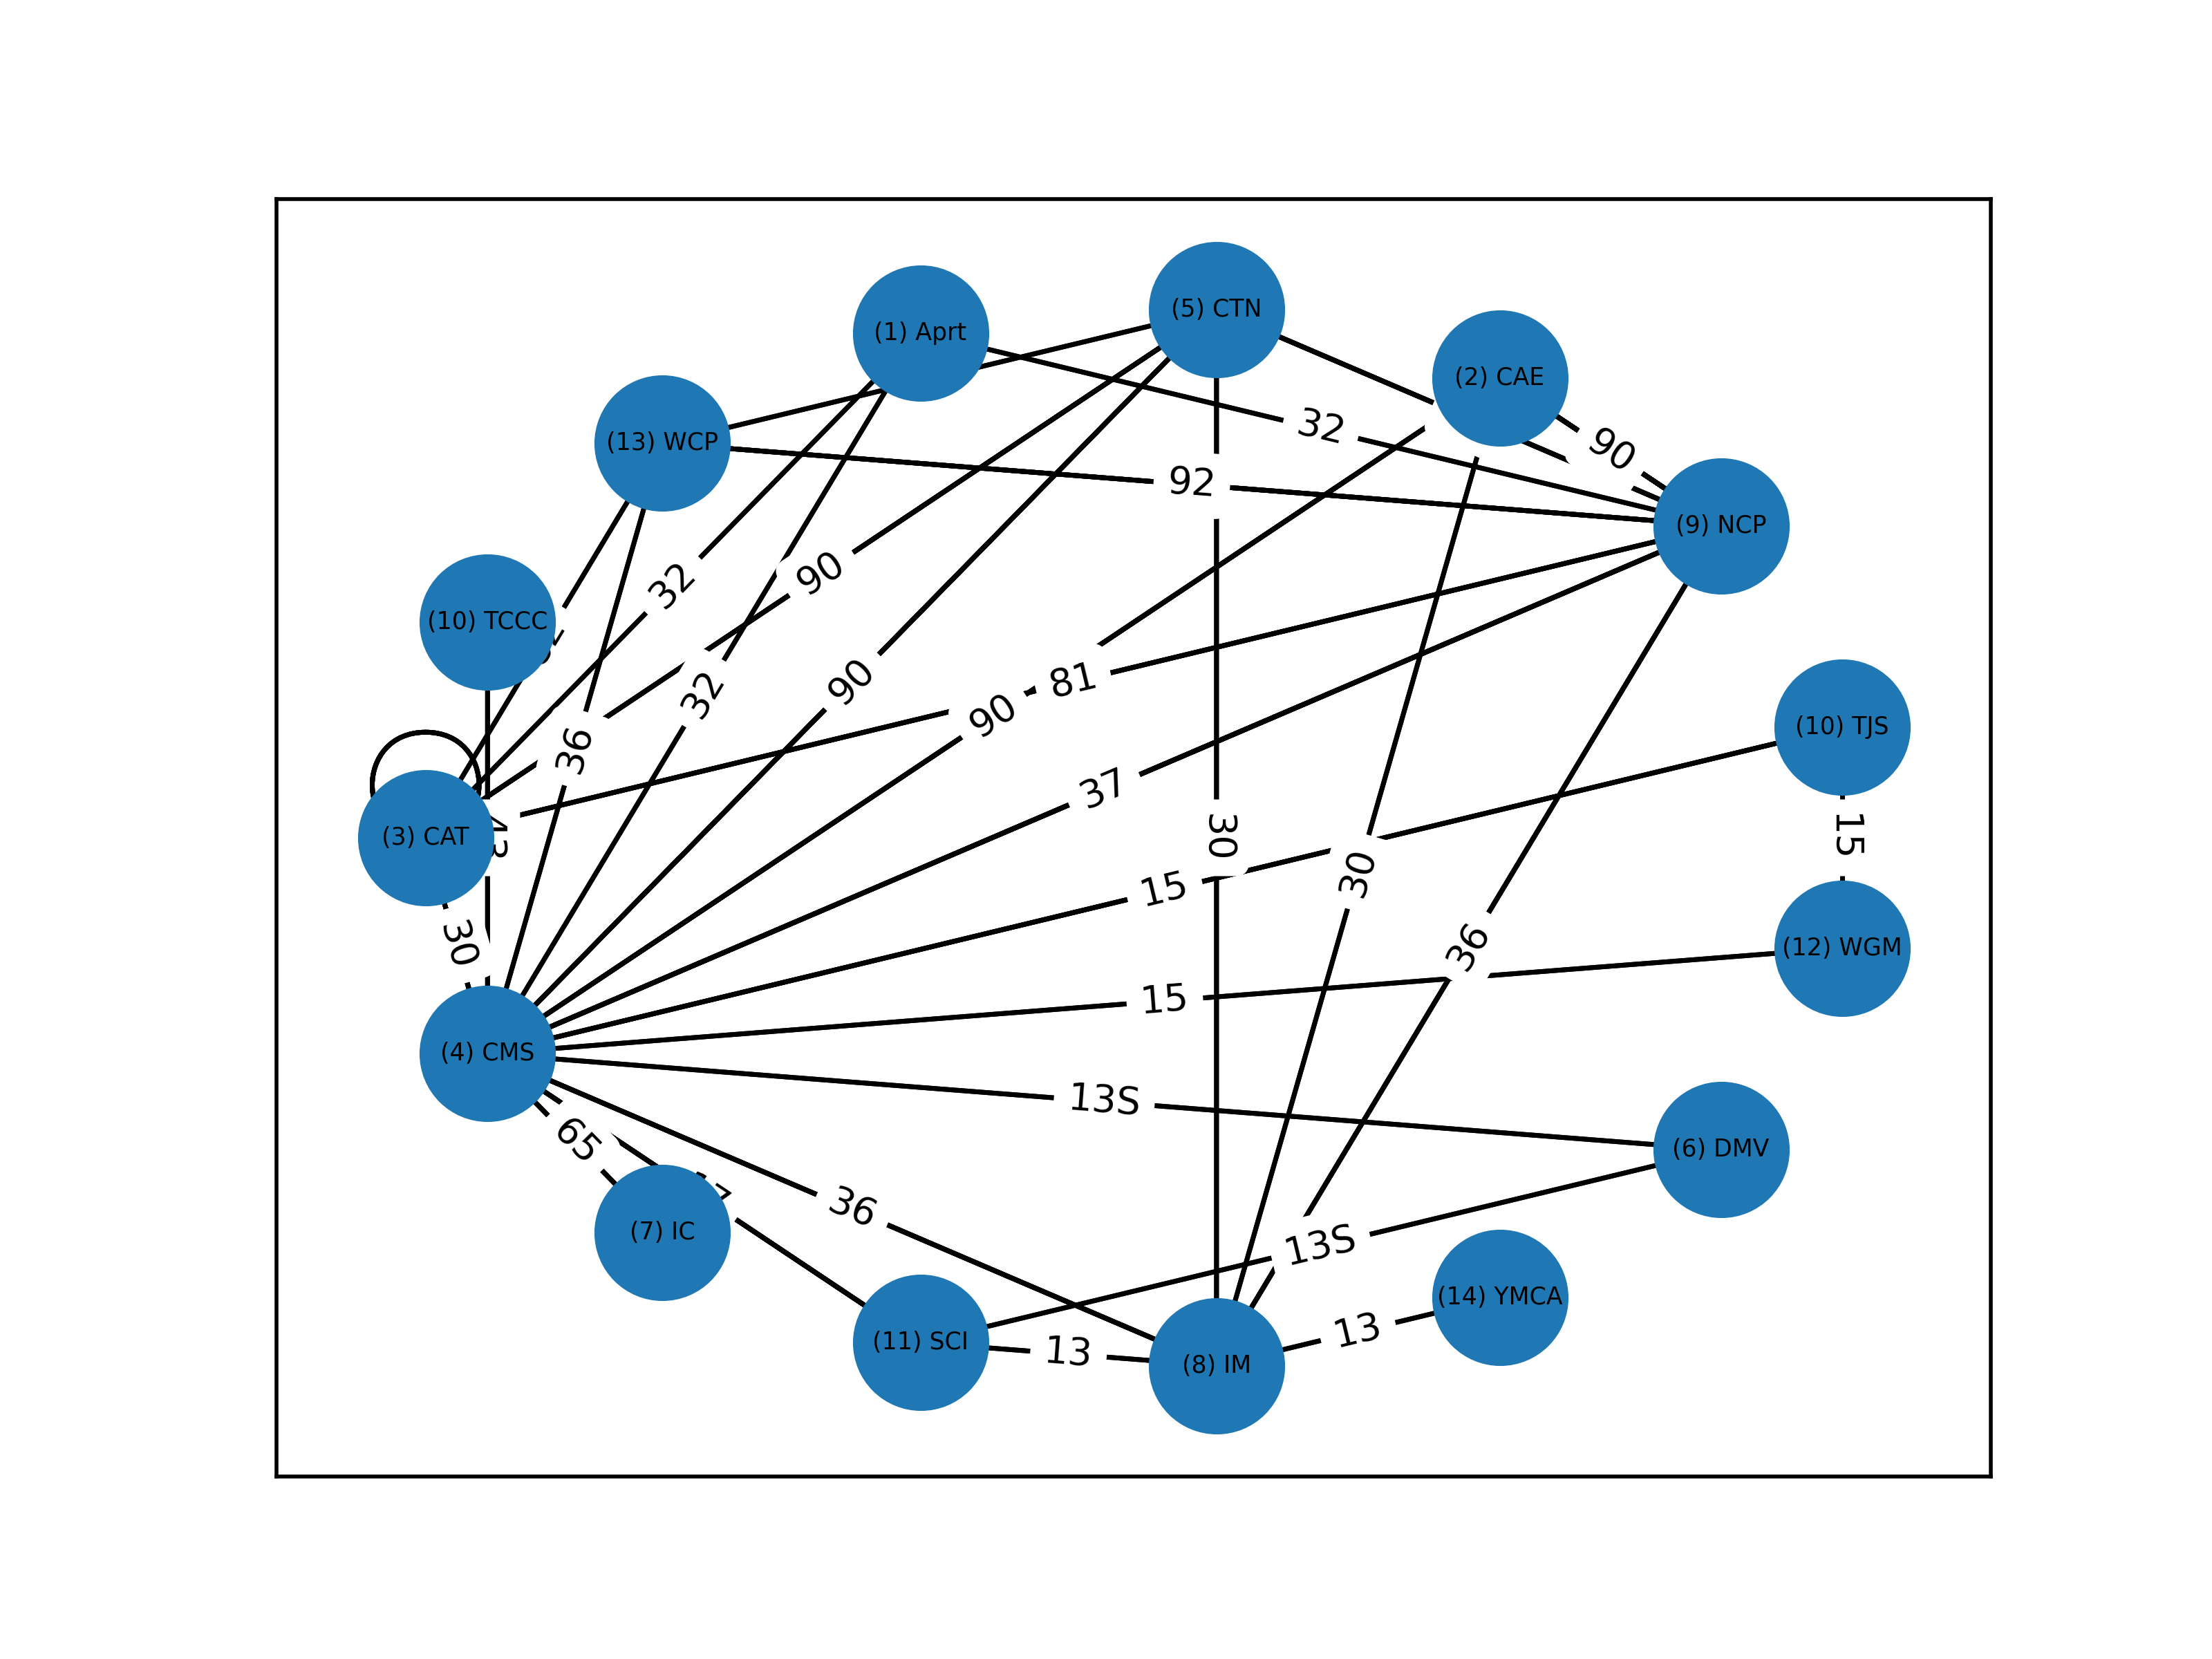
\includegraphics[width=8cm]{TCAT System Shell Layout.png}
\centering
\end{figure}

\[ 
L=
\begin{bmatrix} 
3&0&0&1&0&0&0&0&1&0\\
0&5&3&5&4&0&0&2&6&1\\
0&3&5&1&1&0&0&0&1&0\\
1&5&1&13&3&1&2&3&5&1\\
0&4&1&3&5&0&0&0&2&0\\
0&0&0&1&0&2&0&0&0&0\\
0&0&0&2&0&0&1&0&0&0\\
0&2&0&3&0&0&0&6&2&0\\
1&6&1&5&2&0&0&2&7&0\\
0&1&0&1&0&0&0&0&0&1\\
\end{bmatrix}
\]


\section {Fiedler Eigenvector, Eigenvalue, and Fiedler Set}
We understand visually that the network is complete, therefore no edges must be added. As such, the Fiedler value $\lambda_2=$ is greater than zero and the multiplicity of the eigenvalue of 0 is 1. 
\\
Using the Julia programming language, we find that $\lambda_2=0.3660$ We also compute the corresponding Fiedler vector $v_2$ and list it below. 
\[
v_2=
\begin{bmatrix}
-0.089&
-0.12&
0.044&
0.28&
-0.06&
-0.17&
-0.89&
-0.09&
-0.05&
-0.25
\end{bmatrix}
\]
Accounting for all positive vectors, the resulting Fiedler set is as follows:
\[This is a set
\]

\section{Analysis and Discussion}
Some analysis\\

This project, including the Python program, Julia script, and spreadsheets were uploaded to \href{https://github.com/Ming-DeMers/TCAT-Network-and-Fiedler-Set-Project}{GitHub here.} 

\end{document}
